

\tikzset{every picture/.style={line width=0.75pt}} %set default line width to 0.75pt        

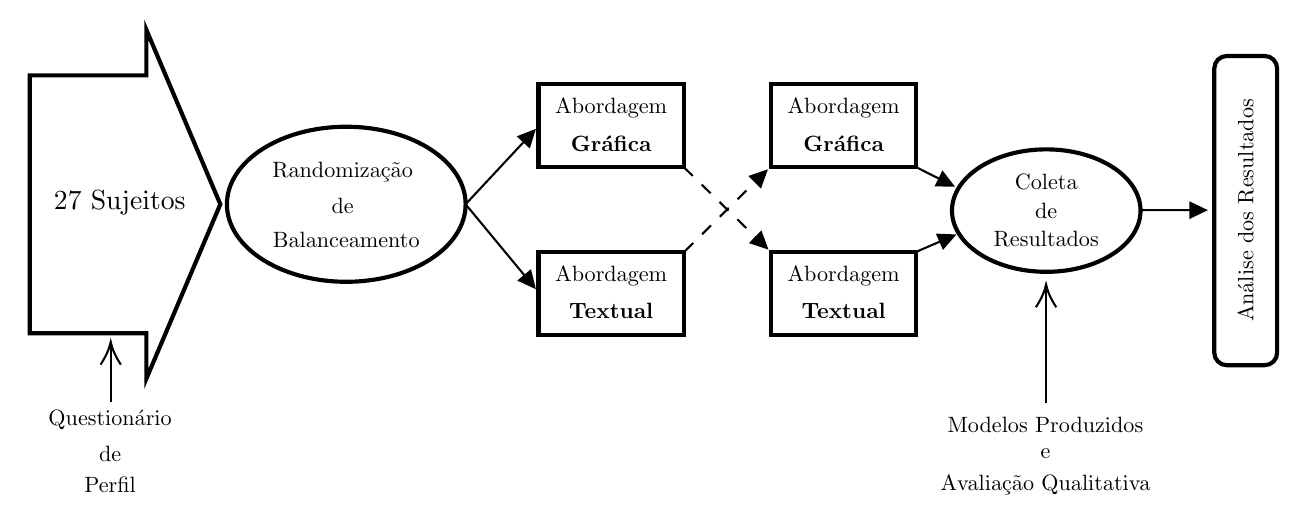
\begin{tikzpicture}[x=0.75pt,y=0.75pt,yscale=-1,xscale=1]
%uncomment if require: \path (0,327.1999969482422); %set diagram left start at 0, and has height of 327.1999969482422




%Shape: Ellipse [id:dp6331487904311781] 
\draw  [line width=1.5]  (448.63,88.9) .. controls (448.63,72.61) and (468.97,59.4) .. (494.05,59.4) .. controls (519.13,59.4) and (539.46,72.61) .. (539.46,88.9) .. controls (539.46,105.19) and (519.13,118.4) .. (494.05,118.4) .. controls (468.97,118.4) and (448.63,105.19) .. (448.63,88.9) -- cycle ;


%Shape: Rectangle [id:dp03801896284105699] 
\draw  [line width=1.5]  (249.43,28) -- (319.43,28) -- (319.43,68) -- (249.43,68) -- cycle ;

%Shape: Ellipse [id:dp583213096835353] 
\draw  [line width=1.5]  (99.3,85.85) .. controls (99.3,65.22) and (125.04,48.5) .. (156.8,48.5) .. controls (188.56,48.5) and (214.3,65.22) .. (214.3,85.85) .. controls (214.3,106.48) and (188.56,123.2) .. (156.8,123.2) .. controls (125.04,123.2) and (99.3,106.48) .. (99.3,85.85) -- cycle ;

%Straight Lines [id:da1799424135415575] 
\draw    (214.3,85.85) -- (246.81,50.98) ;
\draw [shift={(248.17,49.52)}, rotate = 493] [fill={rgb, 255:red, 0; green, 0; blue, 0 }  ][line width=0.75]  [draw opacity=0] (8.93,-4.29) -- (0,0) -- (8.93,4.29) -- cycle    ;

%Straight Lines [id:da17029537209985257] 
\draw    (214.3,85.85) -- (246.9,125.23) ;
\draw [shift={(248.17,126.77)}, rotate = 230.38] [fill={rgb, 255:red, 0; green, 0; blue, 0 }  ][line width=0.75]  [draw opacity=0] (8.93,-4.29) -- (0,0) -- (8.93,4.29) -- cycle    ;

%Straight Lines [id:da39402523544663426] 
\draw  [dash pattern={on 4.5pt off 4.5pt}]  (319.71,108.71) -- (358.51,70.41) ;
\draw [shift={(359.93,69)}, rotate = 495.36] [fill={rgb, 255:red, 0; green, 0; blue, 0 }  ][line width=0.75]  [draw opacity=0] (8.93,-4.29) -- (0,0) -- (8.93,4.29) -- cycle    ;

%Straight Lines [id:da7992081880522388] 
\draw  [dash pattern={on 4.5pt off 4.5pt}]  (319.43,68) -- (358.78,106.32) ;
\draw [shift={(360.21,107.71)}, rotate = 224.24] [fill={rgb, 255:red, 0; green, 0; blue, 0 }  ][line width=0.75]  [draw opacity=0] (8.93,-4.29) -- (0,0) -- (8.93,4.29) -- cycle    ;

%Right Arrow [id:dp4964522106990972] 
\draw  [line width=1.5]  (4.3,23.74) -- (60.47,23.74) -- (60.47,1.77) -- (96.12,85.85) -- (60.47,169.92) -- (60.47,147.96) -- (4.3,147.96) -- cycle ;

%Shape: Rectangle [id:dp003852149638719382] 
\draw  [line width=1.5]  (361.43,28) -- (431.43,28) -- (431.43,68) -- (361.43,68) -- cycle ;

%Shape: Rectangle [id:dp0126542660109914] 
\draw  [line width=1.5]  (361.43,108.75) -- (431.43,108.75) -- (431.43,148.75) -- (361.43,148.75) -- cycle ;

%Shape: Rectangle [id:dp4954877903085966] 
\draw  [line width=1.5]  (249.43,108.75) -- (319.43,108.75) -- (319.43,148.75) -- (249.43,148.75) -- cycle ;
%Straight Lines [id:da3442884963113835] 
\draw    (431.43,68) -- (448.31,76.5) ;
\draw [shift={(450.1,77.4)}, rotate = 206.72] [fill={rgb, 255:red, 0; green, 0; blue, 0 }  ][line width=0.75]  [draw opacity=0] (8.93,-4.29) -- (0,0) -- (8.93,4.29) -- cycle    ;

%Straight Lines [id:da6883068419855551] 
\draw    (431.43,108.75) -- (448.93,101.19) ;
\draw [shift={(450.77,100.4)}, rotate = 516.65] [fill={rgb, 255:red, 0; green, 0; blue, 0 }  ][line width=0.75]  [draw opacity=0] (8.93,-4.29) -- (0,0) -- (8.93,4.29) -- cycle    ;

%Rounded Rect [id:dp5928061300931144] 
\draw  [line width=1.5]  (575,20.46) .. controls (575,17.11) and (577.71,14.4) .. (581.06,14.4) -- (599.24,14.4) .. controls (602.59,14.4) and (605.3,17.11) .. (605.3,20.46) -- (605.3,157.34) .. controls (605.3,160.69) and (602.59,163.4) .. (599.24,163.4) -- (581.06,163.4) .. controls (577.71,163.4) and (575,160.69) .. (575,157.34) -- cycle ;

%Straight Lines [id:da6932528701926595] 
\draw    (539.46,88.7) -- (569.92,88.68) ;
\draw [shift={(571.92,88.68)}, rotate = 539.96] [fill={rgb, 255:red, 0; green, 0; blue, 0 }  ][line width=0.75]  [draw opacity=0] (8.93,-4.29) -- (0,0) -- (8.93,4.29) -- cycle    ;

%Straight Lines [id:da7950818392289087] 
\draw    (43.3,181.2) -- (43.3,154.2) ;
\draw [shift={(43.3,152.2)}, rotate = 450] [color={rgb, 255:red, 0; green, 0; blue, 0 }  ][line width=0.75]    (10.93,-4.9) .. controls (6.95,-2.3) and (3.31,-0.67) .. (0,0) .. controls (3.31,0.67) and (6.95,2.3) .. (10.93,4.9)   ;

%Straight Lines [id:da5784112946450906] 
\draw    (493.97,181.53) -- (493.97,126.53) ;
\draw [shift={(493.97,124.53)}, rotate = 450] [color={rgb, 255:red, 0; green, 0; blue, 0 }  ][line width=0.75]    (10.93,-4.9) .. controls (6.95,-2.3) and (3.31,-0.67) .. (0,0) .. controls (3.31,0.67) and (6.95,2.3) .. (10.93,4.9)   ;


% Text Node
\draw (47.67,85) node  [align=left] {27 Sujeitos};
% Text Node
\draw (156.8,70) node [scale=0.8] [align=left] {Randomização };
% Text Node
\draw (156.8,86.5) node [scale=0.8] [align=left] {de };
% Text Node
\draw (156.8,103) node [scale=0.8] [align=left] {Balanceamento};
% Text Node
\draw (284.43,56.5) node [scale=0.8] [align=left] {\textbf{Gráfica}};
% Text Node
\draw (284.43,39.5) node [scale=0.8] [align=left] {Abordagem};
% Text Node
\draw (396.43,39.5) node [scale=0.8] [align=left] {Abordagem};
% Text Node
\draw (396.43,56.5) node [scale=0.8] [align=left] {\textbf{Gráfica}};
% Text Node
\draw (396.43,120.25) node [scale=0.8] [align=left] {Abordagem};
% Text Node
\draw (396.43,137.25) node [scale=0.8] [align=left] {\textbf{Textual}};
% Text Node
\draw (284.43,120.25) node [scale=0.8] [align=left] {Abordagem};
% Text Node
\draw (284.43,137.25) node [scale=0.8] [align=left] {\textbf{Textual}};
% Text Node
\draw (494.05,75.15) node [scale=0.8] [align=left] {Coleta};
% Text Node
\draw (494.05,88.9) node [scale=0.8] [align=left] {de};
% Text Node
\draw (494.05,102.65) node [scale=0.8] [align=left] {Resultados};
% Text Node
\draw (590.15,88.9) node [scale=0.8,rotate=-270] [align=left] {Análise dos Resultados};
% Text Node
\draw (43,190) node [scale=0.8] [align=left] {Questionário};
% Text Node
\draw (43,206) node [scale=0.8] [align=left] {de};
% Text Node
\draw (43,221) node [scale=0.8] [align=left] {Perfil};
% Text Node
\draw (493.67,221) node [scale=0.8] [align=left] {Avaliação Qualitativa};
% Text Node
\draw (493.67,206) node [scale=0.8] [align=left] {e};
% Text Node
\draw (493.67,192) node [scale=0.8] [align=left] {Modelos Produzidos};


\end{tikzpicture}
